%!TEX root = ..\Main.tex
\section{Results}\todo{TJEK OM DETTE ER TILFÆLDET FOR ALT DET DER ER SKREVET}

%\begin{figure}[h!]
%  \begin{minipage}[t]{0.5\textwidth}
%    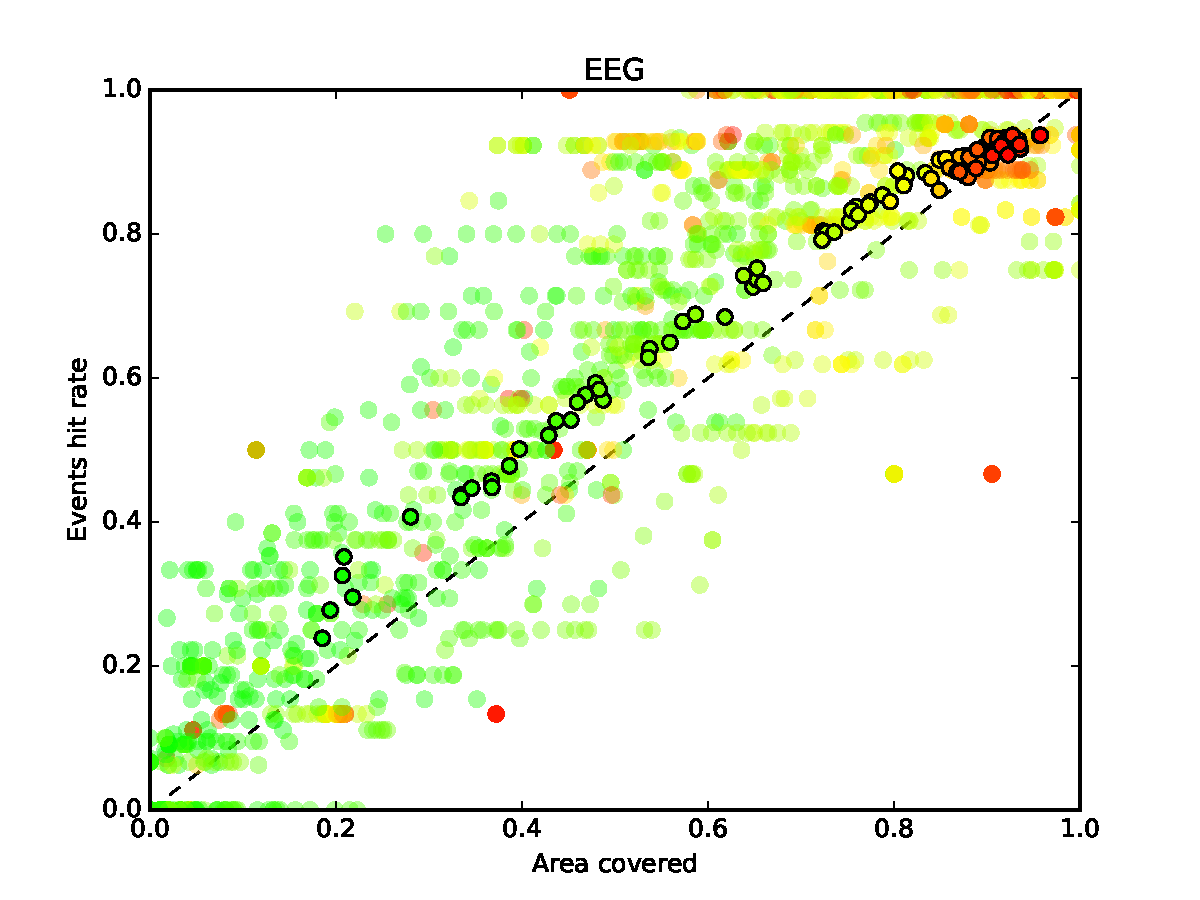
\includegraphics[width=\linewidth,keepaspectratio=true]{graphics/graphs/short/area_covered-events_hit_rate-CovNu-EEG.pdf}
%    \caption{Figura experimental}
%    \label{fase1}
%  \end{minipage}
%  \hspace*{\fill} % it's important not to leave blank lines before and after this command
%  \begin{minipage}[t]{0.5\textwidth}
%    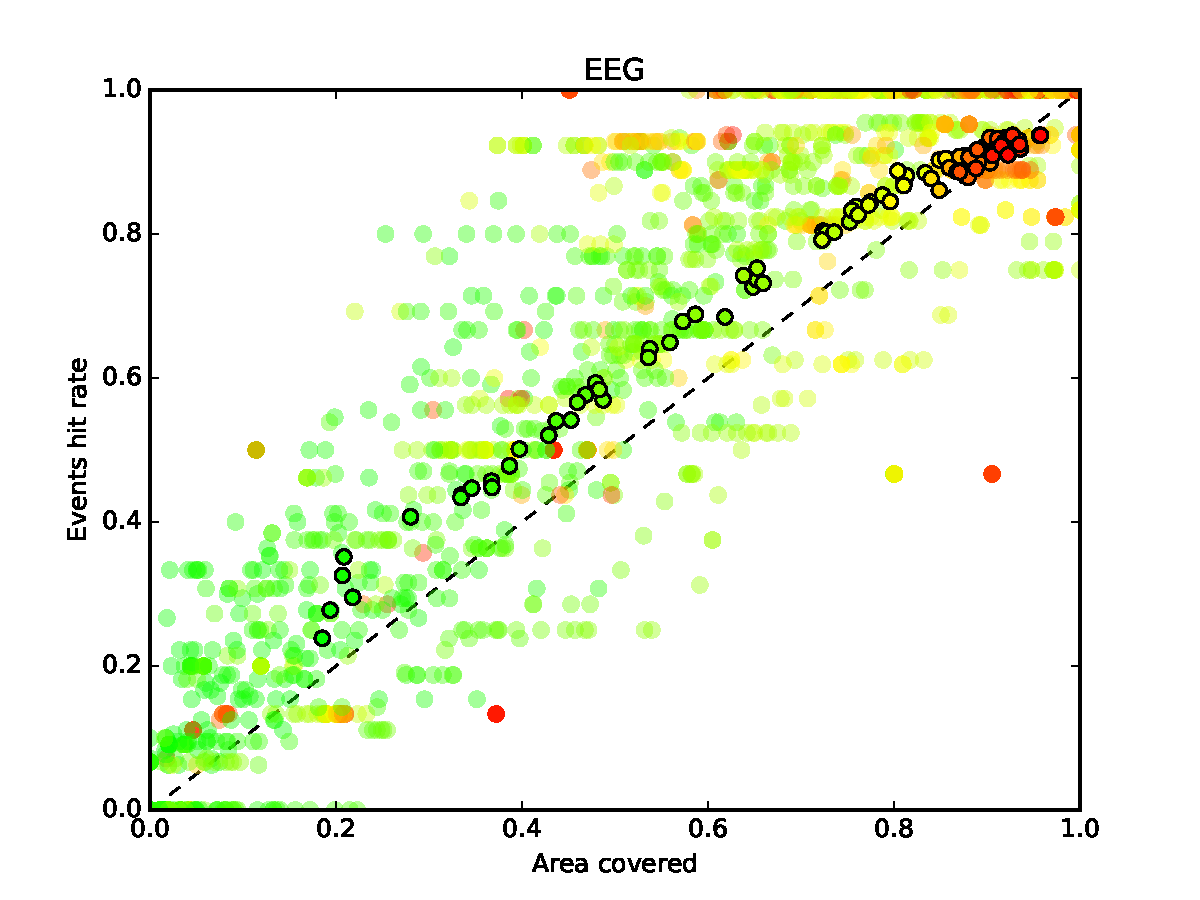
\includegraphics[width=\linewidth,keepaspectratio=true]{graphics/graphs/short/area_covered-events_hit_rate-CovNu-EEG.pdf}
%    \caption{Altra figura experimental}
%    \label{fase2}
%  \end{minipage}
%\end{figure}

\textit{Sensors likeness and differences}\\
In general all the sensor showed the same tendencies....
As seen in Figure x,x,x and x, sensor (x-x) all show that the precision seem steady across the different Nu values with exception of the ones close to 1 seem to decay in their precision. Meaning if you want a classifier that has a reasonable precision but with false positives, a lower Nu value would be applicable.
However looking at Figure x.x.x, and x it can be seen that choosing a higher Nu value for your classifier can yield interesting propositions if the classifier should cover as many problems as possible, however too high a Nu value would cause FCR to be come very high.
%pick some graphs to show where they're very similar
%Something with precision and events hit
%differences
%pick some instances where they are very different!


\textit{Scoring Function likeness and difference}
Looking at the graphs from the two different scoring functions we find that they in general shows the same tendencies, however in x-x these differences can be seen. 
%pick some graphs to show where they're very similar
%differences
%pick some instances where they are very different!